%%%%%%%%%%%%%%%%%%%%%%%%%%%%%%%%%%%%%%%%%%%%%%%%%%%%%%%%%%%%%%%%%%%%%%%%%%%%%%%%%
%
% Purpose:  Top level document for \ThermalRiderDesc.  DO NOT EDIT!!!
%
%
%
%%%%%%%%%%%%%%%%%%%%%%%%%%%%%%%%%%%%%%%%%%%%%%%%%%%%%%%%%%%%%%%%%%%%%%%%%%%%%%%%


\documentclass[twoside,11pt,titlepage]{report}

%
% Bring in the AMS math package
%
\usepackage{amsmath}

%
% Bring in the common page setup
%
\usepackage{dynenv}

%
% Bring in the model-specific commands
%
\usepackage{thermal_rider}

%
% Bring in the graphics environment
%
\usepackage{graphicx}

%
% Bring in the hyper ref environment
%
\usepackage[colorlinks,plainpages=false]{hyperref}
%  keywords for pdfkeywords are separated by commas
\hypersetup{
   pdftitle={\ThermalRiderDesc},
   pdfauthor={\ModelAuthor},
   pdfkeywords={\ModelKeywords},
   pdfsubject={\ThermalRiderDesc}}

\begin{document}

%%%%%%%%%%%%%%%%%%%%%%%%%%%%%%%%%%%
% Front matter
%%%%%%%%%%%%%%%%%%%%%%%%%%%%%%%%%%%
\pagenumbering{roman}

\docid{models/interactions/thermal\_rider}
\docrev{1.0}
\date{\RELEASEMONTH\ \RELEASEYEAR}
\modelname{\ThermalRiderDesc}
\doctype{}
\author{\ModelAuthor}
\managers{
  Robert O. Shelton \\ Project Manager \\
  Michael T. Red \\ Simulation and Graphics Branch Chief \\
  R. Matt Ondler \\ Software, Robotics, and Simulation Division Chief}
\pdfbookmark{Title Page}{titlepage}
\makeDynenvTitlepage

\pdfbookmark{Abstract}{abstract}
%%%%%%%%%%%%%%%%%%%%%%%%%%%%%%%%%%%%%%%%%%%%%%%%%%%%%%%%%%%%%%%%%%%%%%%%%%%%%%%%%
%
% Purpose:  Abstract for the ThermalRider model
%
% 
%
%%%%%%%%%%%%%%%%%%%%%%%%%%%%%%%%%%%%%%%%%%%%%%%%%%%%%%%%%%%%%%%%%%%%%%%%%%%%%%%%


\begin{abstract}

The \ThermalRiderDesc\ is not a stand-alone model; it requires some connectivity to another Interaction model that defines an Interaction Surface (e.g. Radiation Pressure, or Aerodynamic Drag).  Its connection to the Surface Model is indirect, seen only through the Interaction Surface, not the surface itself.

The \ThermalRiderDesc\ serves to provide any Interaction Surface with thermal monitoring capabilities.  Given the current environment, it integrates the thermal processes (e.g. internal power dump, skin friction, radiative absorption, thermal emission) using an R-K 4th order integrator to give the temperature evolution of the surface.


\end{abstract}


\pdfbookmark{Contents}{contents}
\tableofcontents
\vfill

\pagebreak

%%%%%%%%%%%%%%%%%%%%%%%%%%%%%%%%%%%
% Main Document Body
%%%%%%%%%%%%%%%%%%%%%%%%%%%%%%%%%%%
\pagenumbering{arabic}


\setcounter{chapter}{0}

%----------------------------------
\chapter{Introduction}\hyperdef{part}{intro}{}\label{ch:intro}
%----------------------------------

\section{Purpose and Objectives of the \ThermalRiderDesc}
%%%%%%%%%%%%%%%%%%%%%%%%%%%%%%%%%%%%%%%%%%%%%%%%%%%%%%%%%%%%%%%%%%%%%%%%%%%%%%%%%
%
% Purpose:  Introduction for the ThermalRider model.
%
% 
%
%%%%%%%%%%%%%%%%%%%%%%%%%%%%%%%%%%%%%%%%%%%%%%%%%%%%%%%%%%%%%%%%%%%%%%%%%%%%%%%%


%\section{Purpose and Objectives of \ThermalRiderDesc}
% Incorporate the intro paragraph that used to begin this Chapter here. 
% This is location of the true introduction where you explain what this model 
% does.

In some circumstances, it is desirable to have a temperature profile (both temporal and spatial) of the vehicle, while in others, it is more important to avoid the computational effort required to maintain that profile.  For this reason, the thermal monitoring capabilities have been included as a separate entity, although without a surface on which to act, thermal monitoring is not possible.

Therefore, the thermal model is provided as an add-on, or a rider, to any other
interaction model.  So, for example, aerodynamic drag can be calculated without
any reference to skin temperature (or where a reference is required, it can be
assigned to a constant value without great loss of precision).  Or, if the user
wishes to observe the effect of drag on the skin temperature, and perhaps then
on the drag profile itself, the Thermal Rider can be added to the Aerodynamic
Drag model.  It must be cautioned, however, that the Thermal Rider Model is not
a stand-alone model; it requires some connectivity to another Interaction Model
that defines an Interaction Surface (e.g. Radiation Pressure, or Aerodynamic
Drag).  Its connection to the Surface Model is indirect, coming only via the
Interaction Surface; it cannot work on a Surface that is not already an
Interaction Surface.  For details on the concept of surfaces and interaction
surfaces, see the
\href{file:\JEODHOME/models/utils/surface_model/docs/surface_model.pdf}{Surface
Model}~\cite{dynenv:SURFACEMODEL} documentation.

In the \JEODid\ release, the Thermal Rider model provides only the capabilities found in previous releases of JEOD, but now with the capability to easily add functionality as needed.  \JEODid\ implementation includes capacity to evaluate the effect of radiation absorption (from the Radiation Pressure model), and the effect of internal vehicular energy sources and sinks.  The extension section of the User's Guide contains suggestions for including effects of facet-to-facet conduction, and of heating resulting from aerodynamic drag.

The thermal evolution is provided by an internal R-K 4th-order integrator, and is independent of the dynamics integration.




\section{Context within JEOD}
The following document is parent to this document:
\begin{itemize}
\item{\href{file:\JEODHOME/docs/JEOD.pdf}
           {\em JSC Engineering Orbital Dynamics}}
			  \cite{dynenv:JEOD}
\end{itemize}

The \ThermalRiderDesc\ forms a component of the \ModelClass\ suite of
models within \JEODid. It is located at
models/\ModelClass/ThermalRider.  It is used primarily by the
\href{file:\JEODHOME/models/interactions/radiation_pressure/docs/radiation_pressure.pdf}{Radiation
Pressure}~\cite{dynenv:RADIATIONPRESSURE} model, where it can be used in
conjunction with radiation pressure, or as a stand-alone model for simply
monitoring temperature.  It may also be used in the
\href{file:\JEODHOME/models/interactions/aerodynamics/docs/aerodynamics.pdf}{Aerodynamic
Drag}~\cite{dynenv:AERODYNAMICS} model.

\section{Documentation History}
%%%%%%%%%%%%%%%%%%%%%%%%%%%%%%%%%%%%%%%%%%%%%%%%%%%%%%%%%%%%%%%%%%%%%%%%%%%%%%%%%
%
% Purpose:  Change history for document for the ThermalRider model
%
% 
%
%%%%%%%%%%%%%%%%%%%%%%%%%%%%%%%%%%%%%%%%%%%%%%%%%%%%%%%%%%%%%%%%%%%%%%%%%%%%%%%%


%\section{Documentation History}
%%% Status of this and only this document.  Any date should be
%relevant to when 
%%% this document was last updated and mention the reason (release,
%bug fix, etc.)
%%% Mention previous history aka JEOD 1.4-5 heritage in this section.

\begin{tabular}{||l|l|l|l|} \hline
 {\bf Author} & {\bf Date} &  {\bf Revision} & {\bf Description} \\ \hline \hline
 Gary Turner & November, 2009 & 1.0  & JEOD2.0.0 release \\ \hline
\end{tabular}



\section{Documentation Organization}
This document is formatted in accordance with the
NASA Software Engineering Requirements Standard~\cite{NASA:SWE}
and is organized into the following chapters:

\begin{description}
%% longer chapter descriptions, more information.

\item[Chapter 1: Introduction] -
This introduction contains four sections; purpose and objective,
context within JEOD, document history, and document organization.

\item[Chapter 2: Product Requirements] -
Describes requirements for the \ThermalRiderDesc.

\item[Chapter 3: Product Specification] -
Describes the underlying theory, architecture, and design of the
\ThermalRiderDesc\ in detail.  It will be organized in
four sections; Conceptual Design, Mathematical Formulations, Detailed
Design, and Version Inventory.

\item[Chapter 4:  User's Guide] -
Describes how to use the \ThermalRiderDesc\ in a Trick simulation.  It
is broken into three sections to represent the JEOD
defined user types; Analysts or users of simulations (Analysis),
Integrators or developers of simulations (Integration),
and Model Extenders (Extension).

\item[Chapter 5: Verification and Validation] -
Contains \ThermalRiderDesc\ verification and validation procedures and
results.

\end{description}


%----------------------------------
\chapter{Product Requirements}\hyperdef{part}{reqt}{}\label{ch:reqt}
%----------------------------------

\requirement{Top-level Requirement}
\label{reqt:top_level}
\begin{description}
\item[Requirement:]\ \newline
  This model shall meet the JEOD project requirements specified in
  the \JEODid\
  \hyperref{file:\JEODHOME/docs/JEOD.pdf}{part1}{reqt}{ top-level
  document}~\cite{dynenv:JEOD}.
\item[Rationale:]\ \newline
  This model shall, at a minimum,  meet all external and
  internal requirements
  applied to the \JEODid\ release.
\item[Verification:]\ \newline
  Inspection \vref{inspect:top_level}
\end{description}


%%%%%%%%%%%%%%%%%%%%%%%%%%%%%%%%%%%%%%%%%%%%%%%%%%%%%%%%%%%%%%%%%%%%%%%%%%%%%%%%%
%
% Purpose:  requirements for the ThermalRider model
%
% 
%
%%%%%%%%%%%%%%%%%%%%%%%%%%%%%%%%%%%%%%%%%%%%%%%%%%%%%%%%%%%%%%%%%%%%%%%%%%%%%%%%

% add text here to describe general model requirements
% text is of the form:
%\requirement{REQUIREMENT DESCRIPTION}
%\label{reqt:REQT_DESC_ABBREVIATED}
%\begin{description}
%  \item[Requirement:]\ \newline
%     <Insert description of requirement> 
%  \item[Rationale:]\ \newline
%     <Insert description of rationale> 
%  \item[Verification:]\ \newline
%     <Insert description of verification (e.g. "Inspection")> 
%\end{description}

\requirement{Temperature Monitoring}
\label{reqt:temp_monitoring}
\begin{description}
  \item[Requirement:]\ \newline
    The \ThermalRiderDesc\ shall provide the capability to monitor the temporal and spatial profiles of the vehicle surface temperatures. 
  \item[Rationale:]\ \newline
    The temperature of a particular area of a vehicle may be of critical importance in the design of the vehicle; variation of temperature across the surface of the vehicle could affect the dynamics of the vehicle in a high fidelity simulation.  Therefore, it is important to be able to identify the temporal temperature profile of certain critical areas of the vehicular surface, and hence the capability to model the spatial variation across the vehicle.
  \item[Verification:]\ \newline
	  Tests \vref{test:temperature_integration1} and \vref{test:temperature_integration2}
\end{description}

\requirement{Minimum Functionality}
\label{reqt:thermal_min_func}
\begin{description}
  \item[Requirement:]\ \newline
    The \ThermalRiderDesc\ shall provide, at a minimum, the ability to accurately represent the effect of radiation absorption and emission.
\item[Rationale:]\ \newline
  Prior to the release of
  \JEODid, the thermal modeling had been an intrinsic part of the radiation-pressure model, which requires knowledge of the temperature-time profile in order to accurately represent the effects of radiation-pressure.  This requirement simply reflects the transfer of responsibility for these calculations from the old radiation model (which incorporated both radiation and thermal modeling) to the new \ThermalRiderDesc.
  \item[Verification:]\ \newline
	  Tests \vref{test:temperature_integration1} and \vref{test:temperature_integration2}
\end{description}

\requirement{Extended Functionality}
\label{reqt:thermal_ext_func}
\begin{description}
  \item[Requirement:]\ \newline
    The \ThermalRiderDesc\ shall, at a minimum, provide the basic architecture to allow future extension to include representation of the effects of:
  \begin{enumerate}
    \item Power sources and sinks from within the vehicle itself.
    \item Facet-to-facet thermal conduction.
    \item Heating resulting from aerodynamic drag.
  \end{enumerate}
\item[Rationale:]\ \newline
  There are many methods by which the temperature of a surface can be altered.  These three, in addition to the effect of radiative absorption and emission, were considered to be the most influential.
  \item[Verification:]\ \newline
	  Inspection \vref{inspect:thermal_ext_func}
\end{description}


\section{Requirements Traceability}\label{sec:traceability}

\begin{longtable}[c]{||p{3in}|p{3in}|}
\caption{Requirements Traceability} \\[6pt]
\hline
{\bf Requirement} & {\bf Inspection and Testing} \\ 
\hline \hline
\endfirsthead
\hline
\endfoot
\caption[]{Requirements Traceability (continued)} \\[6pt]
\hline
{\bf Requirement} & {\bf Inspection and Testing} \\ 
\hline \hline
\endhead
\ref{reqt:top_level} - Top-level Requirements &
  Insp.~\ref{inspect:top_level} \\ \hline

\ref{reqt:temp_monitoring} -  Temperature Monitoring
& Test~\ref{test:temperature_integration1} \\
& Test~\ref{test:temperature_integration2} \\ \hline

\ref{reqt:thermal_min_func} -  Minimum Functionality
& Test~\ref{test:temperature_integration1} \\
& Test~\ref{test:temperature_integration2} \\ \hline

\ref{reqt:thermal_ext_func} -  Extended Functionality
&  Insp.~\ref{inspect:thermal_ext_func} \\ \hline

\end{longtable}



%----------------------------------
\chapter{Product Specification}\hyperdef{part}{spec}{}\label{ch:spec}
%----------------------------------

\section{Conceptual Design}
%%%%%%%%%%%%%%%%%%%%%%%%%%%%%%%%%%%%%%%%%%%%%%%%%%%%%%%%%%%%%%%%%%%%%%%%%%%%%%%%%
%
% Purpose:  Conceptual part of Product Spec for the ThermalRider model
%
% 
%
%%%%%%%%%%%%%%%%%%%%%%%%%%%%%%%%%%%%%%%%%%%%%%%%%%%%%%%%%%%%%%%%%%%%%%%%%%%%%%%%


%\section{Conceptual Design}
This section describes the key concepts found in the \ThermalRiderDesc.
For an
architectural overview, see the 
\href{file:refman.pdf} {\em Reference Manual}
\cite{thermalbib:ReferenceManual}


\subsection{The Rider Hierarchy}
The \ThermalRiderDesc\ requires the definition, in some other model, of an Interaction
Surface, which is an element of the
\href{file:\JEODHOME/models/utils/surface\_model/docs/surface\_model.pdf}{Surface
Model}~\cite{dynenv:SURFACEMODEL}.  For
details on the Surface Model, see the Surface Model Product
Specification.  Presented here is a very cursory overview of the
Surface Model, intended to put the Thermal Rider into context.

Starting with the most general form, the Surface Model comprises a number of Facets; the facets typically have some topology and/or geometry (e.g., flat-plate with some specific area and orientation).  Together, these can be used to describe the geometry of the surface, or can be left as somewhat abstract, disconnected entities.  Each Facet can be further defined to become an Interaction Facet; Interaction Facets contain additional data necessary to know how to interact with some particular environmental factor.

While a generic Surface comprises a number of Facets, the associated Interaction Surface comprises the Interaction Facets associated with each of the Facets in the generic Surface.  The Interaction Surface is an abstract concept that is not really implemented directly; instead specific examples of Interaction Surfaces are created, such as a radiation-pressure surface, or an aerodynamic surface, that are specific to a particular environmental interaction.  Conversely, the generic Surface is simply geometric in nature and applicable to multiple situations. 

Thus, each interaction model (Radiation Pressure, Aerodynamic Drag, other
user-specified models) utilizes an implementation of an interaction surface that comprises a collection of model-specific Interaction Facets (e.g., Radiation Facets).  These model-specific
interaction facets inherit their basic data from the Interaction Facets (i.e.,
those defined in the Interaction Surface Model), and add model-specific values
and methods to simulate the actual interaction between the surface and the
environment.

One of those model-specific members that can be added to each Interaction Facet is a collection
of thermally-related values.
This is called the Thermal-\textit{Facet}-Rider; it is added to each model-specific interaction facet (e.g. Radiation Facet).  To accompany the rider on each facet, there is also a \textit{model} rider that basically instructs the non-thermal instance of the Interaction Model to include thermal effects.  This is called the Thermal-\textit{Model}-Rider (italics used to distinguish between the facet rider and the model rider).

An example of using the Rider concept can be found in the default Radiation Pressure model.  
\begin{quotation}
The class \textit{radiation\_presssure} contains an instance of the \textit{ThermalModelRider}, called \textit{thermal}.
The Radiation Pressure \textit{update} method is called from the
\textit{S\_define}, which calls the
ThermalModelRider \textit{update} method.
That, in turn, calls the Radiation Surface
\textit{thermal\_integrator} method, which cycles through all facets calling each facet's ThermalFacetRider's \textit{integrate} function to integrate the rate of change of temperature.
\end{quotation}

\subsection{Independent Integration}
The standard dynamic integration that takes place behind-the-scenes requires the
input of forces, which are translated into accelerations, and integrated to
provide updated values of velocity and position.  Similarly, torques are
provided for the angular components.  However, those forces and torques depend
on the temperature profile.  Integrating the temperature profile with the
dynamics will lead to unnecessary errors; these can easily be circumvented by independently integrating the temperature prior to calculating the forces that are fed to the dynamics integrator.

Therefore, the \ThermalRiderDesc\ provides the capability to independently integrate the temperature.

\subsection{Handling Multiple Interaction Models}
Both problems and opportunities present themselves when a simulation requires
the consideration of multiple interaction models.

The Thermal Rider Model is always associated with one specific instance of an Interaction Model,
which contains one specific instance of an Interaction Surface -- comprising interaction-specific Interaction Facets --
which are based on the geometric Facets.  Since each Interaction
Model carries its own Interaction Facets, it must carry its own
Thermal-Rider Model for that set of Interaction Facets.  
If each collection of Interaction Facets is based on a common
geometric surface, then it is a straightforward task to direct all thermal
processes to one Interaction Model, and include a
\textit{ThermalModelRider}
for only that model, and \textit{ThermalFacetRider}s for only that set of
Interaction Facets.
In this case, it is recommended that the Radiation Pressure Model (if being used) be the model that is used to contain the Thermal Rider Model, since it is the most closely tied to the temperature.

A more complicated scenario occurs when the different Interaction Models use
different base Facets, such as when different fidelity is required between the
different models.  Here again, it is recommended that only one model carry the
Thermal Rider.  Complications arise when the desired fidelity of the
Thermal-Rider Model is not directly matched with any of the Interaction Surfaces,
or is only matched to one of the non-preferred models.  The solution to this
usually involves changing the desired fidelity on either the Thermal-Rider or one of the
preferred Interaction Models.


%\section{Mathematical Formulations}
%%%%%%%%%%%%%%%%%%%%%%%%%%%%%%%%%%%%%%%%%%%%%%%%%%%%%%%%%%%%%%%%%%%%%%%%%%%%%%%%%
%
% Purpose:  Mathematical Formulation part of Product Spec for the ThermalRider model
%
% 
%
%%%%%%%%%%%%%%%%%%%%%%%%%%%%%%%%%%%%%%%%%%%%%%%%%%%%%%%%%%%%%%%%%%%%%%%%%%%%%%%%

\section{Mathematical Formulations}

\subsection{Basic Equations}

The equation for temperature of a facet is based on an emission-absorption
model.  Thermal emission is modeled using a black-body baseline, modified by the
emissivity of the surface.  The total power, $P$, radiated by a surface
at temperature $T$ and with surface area $A$ is 

\begin{equation}\label{eqn:thermalemission}
P = \epsilon \sigma A T^4 
\end{equation}

where $\epsilon$ is the emissivity of the surface, 
and $\sigma$ is the Stefan-Boltzmann constant, $\sigma = 5.6704004 \times
10^{-8} \ W \; m^{-2} \; K^{-4}$

We model the power absorbed $P_{abs}$ as the sum of the power from external
sources of radiation, thermal input from the vehicle, and as a possible future
extension, conduction from other facets.  The current implementation ignores
conduction.

The net flow of power can be represented as a rate of change of temperature by
factoring in the specific heat of the facet,

\begin{equation}\label{eqn:temperatureODE}
Q \frac{dT}{dt} = P_{abs} - \epsilon \sigma A T^4
\end{equation}

where $Q$ is the specific heat, expressed in  $J \cdot K^{-1}$
and $P_{abs}$is the rate at which energy 
is absorbed into a facet.

\subsection {Temperature Propagation}

 The conventional JEOD approach to solving ~\ref{eqn:temperatureODE} has been
to use a special $4^{th}$ order Runge-Kutta technique which is included in the 
\textit{ThermalFacetRider} class.  This technique includes a series of tests
in order to avoid instabilities resulting from an integration step too large
to accommodate rapidly varying temperatures.

With the introduction of first order methods in the \textit{er7\_utils} package,
it is now possible to have JEOD propagate temperature just as it propagates
the state of a vehicle.  This approach required the introduction of the 
new \textit{ThermalIntegrableObject} class which is derived from
\textit{er7\_utils::IntegrableObject}.  The \textit{integrate} method of
\textit{ThermalIntegrableObject} performs each step of the integration cycle.
This method also checks at each step to make sure that the
equilibrium temperature is not surpassed within an integration cycle.

\subsection{Runge-Kutta 4th Order (RK4) Integrator}\label{ref:thermalRK4integrator}

The rate at which temperature changes is a strong function of
temperature due to the rate of thermal emission, as described 
in equation \ref{eqn:thermalemission}.
It is assumed that other contributing factors change more slowly, 
indeed that they are constant over an integration step.
All other factors are combined into the value \textit{power\_absorb}, which 
is positive if there is a net power into the facet (excluding thermal emission), and negative if there is a net flow out from the surface 
(e.g. from a thermal source within the vehicle).
With those assumptions, the RK4 integrator can be implemented as follows:

$T_0$ represents the initial temperature at the start of the integration step.

The first full-step approximation to the temperature change, $I_1$, is
calculated as 
\begin{equation*}
I_1 = \frac{\Delta t}{Q} \left(  P_{abs} - \epsilon \sigma A T_0^4 \right)
\end{equation*}

The second step uses the mid-point temperature as the operating temperature, calculated as the average of $T_0$ and $T_0 + I_1$.   
\begin{equation*}
T_1 = T_0 + \frac{I_1}{2}
\end{equation*}
\begin{equation*}
I_2 = \frac{\Delta t}{Q} \left(  P_{abs} - \epsilon \sigma A \left(T_1 \right) ^4 \right)
\end{equation*}

The third step uses the mid-point temperature, calculated as the
average of $T_0$ and $T_0 + I_2$ as the operating temperature,  
\begin{equation*}
T_2 = T_0 + \frac{I_2}{2}
\end{equation*}
\begin{equation*}
I_3 = \frac{\Delta t}{Q} \left(  P_{abs} - \epsilon \sigma A \left(T_2 \right) ^4 \right)
\end{equation*}

The  fourth step uses the predicted end value, $T_0 + I_3$ as the
operating temperature,  
\begin{equation*}
T_3 = T_0 + I_3
\end{equation*}
\begin{equation*}
I_4 = \frac{\Delta t}{Q} \left(  P_{abs} - \epsilon \sigma A \left(T_3 \right) ^4 \right)
\end{equation*}

The actual change in temperature is then calculated as a weighted average of those 4 values,
\begin{equation*}
\Delta T = \frac{I_1+2I_2+2I_3+I_4}{6}
\end{equation*}

\subsubsection{Integrating close to the asymptote}
If the integration time-step is large compared to the characteristic time over
which the temperature can change appreciably, there is the potential that the
RK4 integrator can become unstable.  This is due to the asymptotic nature of the
temperature$\sim$time evolution; whether the temperature is above or below the
equilibrium temperature, the temperature will asymptotically approach equilibrium.  The instability is observed when the integration time-step is
sufficiently large that the local
linearization of that asymptotic approach jumps over the asymptote in one step,
and then tries to approach from the other side.

Figure \ref{fig:tempasymptote} illustrates the temperature$\sim$time profile, with the asymptotic trend both above and below the asymptote at $T_{eq}$.  Note that the two profiles are not symmetric; the upper profile is a little steeper for the same temperature difference from $T_{eq}$, making this instability more likely when approaching from above than when approaching from below.


\begin{figure}[htp]
\begin{center}
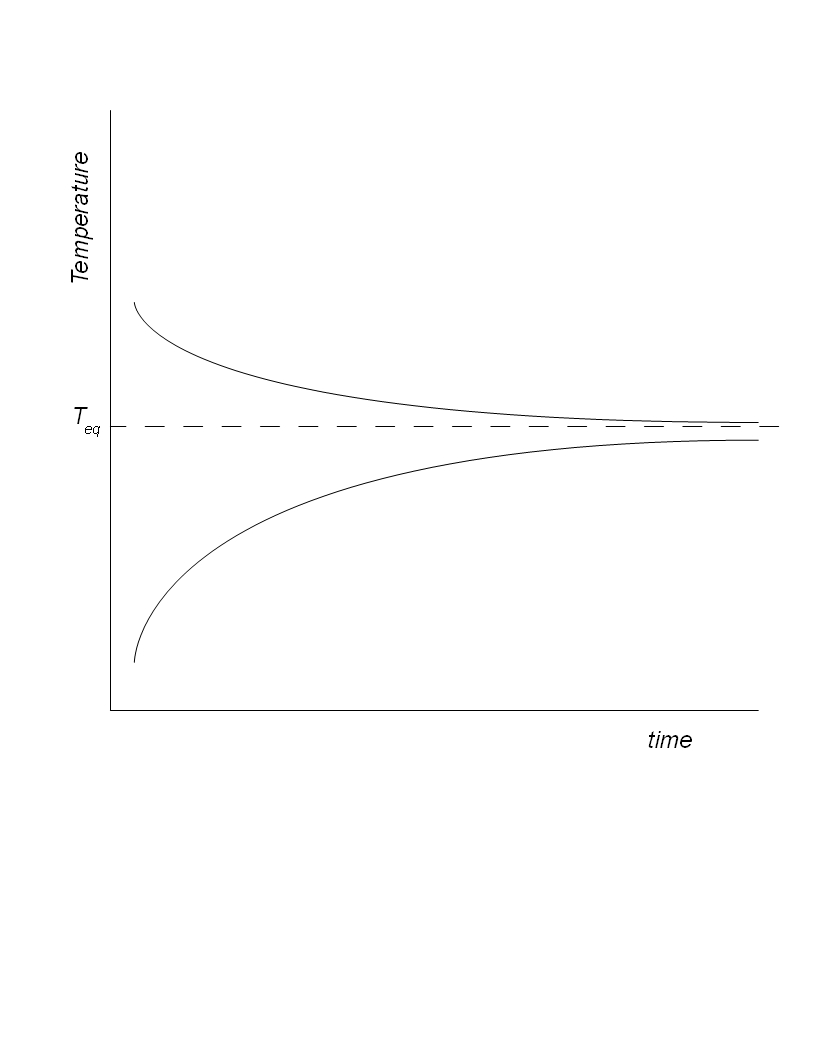
\includegraphics[width=3.2736in,height=2.85in]{figures/temp_integ.jpg}
\caption{Illustration of the temperature$\sim$time profile near the equilibrium temperature.}
\label{fig:tempasymptote}
\end{center}
\end{figure}

\begin{quotation}
Aside:  The rate at which the surface radiates energy is $P_{rad} \propto T^4$.

The rate at which the surface absorbs energy is some constant $P_{abs}$.  

At equilibrium, these two are equivalent,  $P_{abs} = P_{rad} \propto {T_{eq}}^4$.


The net rate at which energy increases is therefore
\begin{equation*}
\epsilon = (P_{abs} - P_{rad}) \propto \frac{dT}{dt}.
\end{equation*}  

Therefore, 
\begin{equation*}
\frac{dT}{dt} \propto ({T_{eq}}^4 - T^4).
\end{equation*}  

Then for some deviation from the equilibrium temperature:
\begin{equation*}
T=T_{eq}+\Delta T \Rightarrow \frac{dT}{dt} \propto 
(-) \left( T_{eq} \right)^4 
\left(
4 \left( \frac{\Delta T}{T_{eq}} \right) + 
6 \left( \frac{\Delta T}{T_{eq}} \right)^2 + 
4 \left( \frac{\Delta T}{T_{eq}} \right)^3 + 
  \left( \frac{\Delta T}{T_{eq}} \right)^4 
\right)
\end{equation*}  

The difference between above the asymptote and below the asymptote results from the sign change on $\Delta T$.  The first and third terms will have different signs for the two cases, whereas the second and fourth will have the same sign regardless of whether the temperature is above or below the asymptote.  The consequence is that above the asymptote, all terms are additive, and below the asymptote the terms tend to cancel each other.

\end{quotation}

Figure \ref{fig:tempasymptote1} illustrates the problem with having an
integration time-step that is too large.  In the first step, the original
temperature ($T_0$) is used to calculate the rate of change of temperature, and
the predicted change to that temperature ($I_1$).  Next, that change is used to
derive an intermediate temperature ($T_1 = T_0 + 0.5 I_1$), which is below the
asymptote.  This temperature is used to calculate a new temperature gradient
which is now positive; that temperature gradient is used to calculate a new
correction ($I_2$, not shown) to the original temperature.  The next
intermediate temperature ($T_2 = T_0 + 0.5 I_2$) will then be higher than $T_0$,
therefore have a steeper gradient, which leads to $I_3$ having a larger
deviation than did $I_1$.  Thus, the calculation of $T_3 = T_0 + I_3$ falls far
below the equilibrium value, which is highly erroneous, and further leads to a
ridiculously large value for $I_4$.  The consequence is that the temperature
change could be driven to non-physical values, and in the opposite direction to which it should have been evolving.

\begin{figure}[htp]
\begin{center}
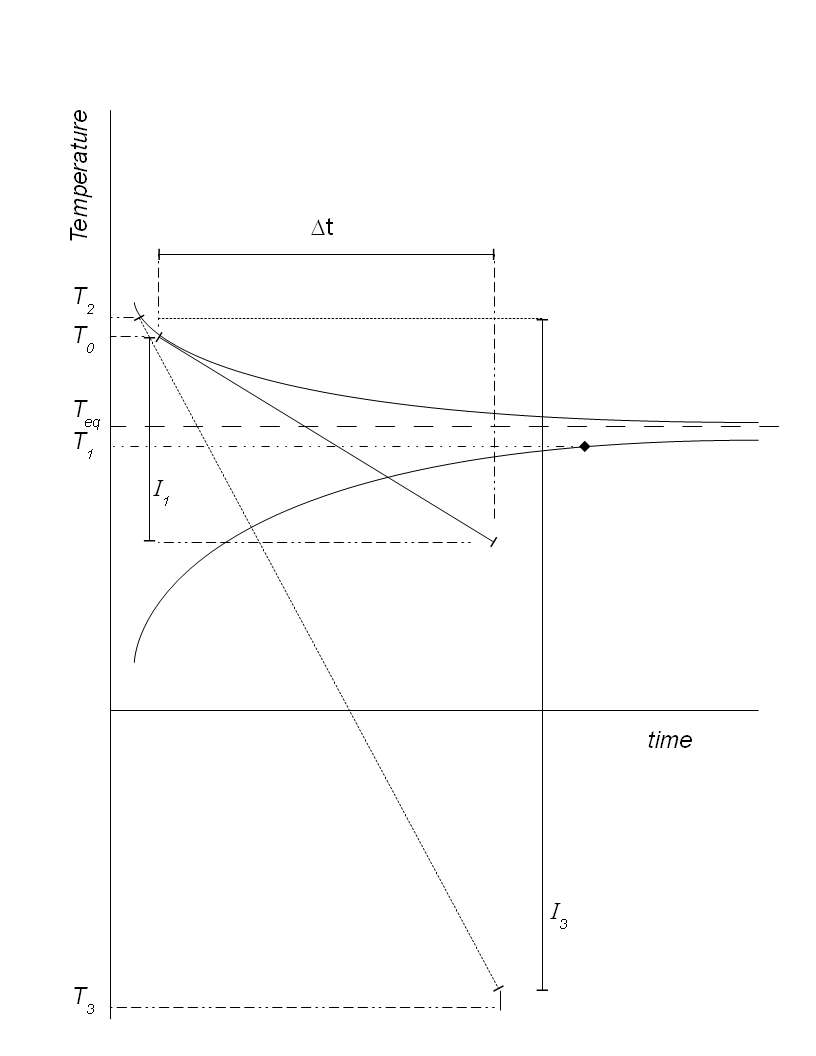
\includegraphics[height=200mm]{figures/temp_integ1.jpg}
\caption{Illustration of the instability near the equilibrium temperature.}
\label{fig:tempasymptote1}
\end{center}
\end{figure}

To prevent this instability, there are numerous checks made during the integration.  First, the direction of anticipated temperature change is recorded as \textit{dt\_dir} ($\pm 1$ corresponding to up and down) by comparing the original temperature to the equilibrium temperature.

Next, $I_1$ is calculated; it is assumed that $I_1$ has the correct direction to it.  $I_1$ is used to calculate $T_1$ and thereby $I_2$, the latter of which is compared against \textit{dt\_dir} to ensure that it is in the correct direction.  If this is not the case, the predicted temperature is set to the equilibrium temperature and the integration ends.

The same check could be made on $I_3$, but it is not necessary.  Since $T_1$ is closer than $T_0$ to $T_{eq}$, the magnitude of $I_2$ must be less than the magnitude of $I_1$.  Therefore, if $I_1$ was insufficient to cross the asymptote, $I_2$ must have been likewise; hence if $I_2$ was in the correct direction, $I_3$ must also be in the correct direction.

The same is not true of $I_4$, since $T_3$ uses a full-step correction to $T_0$, whereas $T_1$ and $T_2$ used only half-step corrections.  $T_3$ could, therefore, be on the wrong side of the equilibrium temperature.  Incorporating $I_4$ in this situation would lead to a calculated temperature change that is too small; ignoring it would lead to the value being too large, and the final temperature being very close to equilibrium.  Instead, one-half of the value is taken.

The four temperature deviations are combined then to give the final temperature change.

Once again, checks are made that this is sensible.  If the temperature change was in the wrong direction (this may be impossible), or if the temperature change results in a new temperature that is on the wrong side of equilibrium (this, too, may be impossible) the temperature is set to the equilibrium temperature.




\subsection{Emitted Power}
The mean emitted power over the integration step can now be calculated from the resulting change to the temperature.

\begin{equation}
P_{emit} = Q\frac{ \Delta T}{\Delta t} - P_{abs}
\end{equation}

Note: a positive value of $P_{emit}$ means that the facet gains
energy by emission (physically impossible).  $P_{emit}$ is typically negative.

%\section{Detailed Design}

%%%%%%%%%%%%%%%%%%%%%%%%%%%%%%%%%%%%%%%%%%%%%%%%%%%%%%%%%%%%%%%%%%%%%%%%%%%%%%%%%
%
% Purpose:  Detailed part of Product Spec for the ThermalRider model
%
% 
%
%%%%%%%%%%%%%%%%%%%%%%%%%%%%%%%%%%%%%%%%%%%%%%%%%%%%%%%%%%%%%%%%%%%%%%%%%%%%%%%%

\section{Detailed Design}

This section is divided into 2 parts:


\begin{itemize}
\item A process flow-through description, or Process Architecture of the sequence in which the
various functions are called, and the interaction between the objects.
\item An alphabetized list of the objects that comprise the
\ThermalRiderDesc, 
with reference to the parent class where appropriate, and description
of the functions contained within those object.
\end{itemize}

Further, the 
\href{file:refman.pdf} {\em Reference Manual} \cite{thermalbib:ReferenceManual}
contains a
structural overview of the \ThermalRiderDesc.

\subsection{Process Architecture}

\subsubsection{Initialization}

The initialization of the \ThermalRiderDesc\ starts with the implementation of the generic aspects of the Interaction Model (on which the \ThermalRiderDesc\ rides):
\begin{enumerate}
\item The Interaction Surface is created. 
\item The specific Interaction Model is initialized.  
\end{enumerate}
For specific information on these processes, see
the appropriate documents (
  \href{file:\JEODHOME/models/utils/surface\_model/docs/surface\_model.pdf}{Surface
  Model}\cite{dynenv:SURFACEMODEL} and,
  for example,
  \href{file:\JEODHOME/models/interactions/radiation\_pressure/docs/radiation\_pressure.pdf}{Radiation
  Pressure}\cite{dynenv:RADIATIONPRESSURE}).

\begin{enumerate}
\item  The initialization of the generic Interaction Surface has
little direct impact on this model, it creates the surface for later
population by an Interaction Model.
\item  The initialization of the specific Interaction Model must include the following
tasks:
\begin{enumerate}
\item The \textit{thermal.active} flag must be set (to be \textit{true} or \textit{false}).  If
it is set to false, the \ThermalRiderDesc\ will not be utilized.  The
rest of the initialization proceeds regardless of this flag setting;
this allows the user to switch the flag mid-simulation and still have
the \ThermalRiderDesc\ available immediately.
\item The initialization method for the specific instance of the
Interaction Surface (e.g. Radiation Surface) must be called.

The initialization routine for the surface calls the initialization routine for each facet in that surface, which in turn call the \textref{initialize}{ref:facetinitialize}
routine located in its attached ThermalFacetRider object.  

\end{enumerate}
\end{enumerate}



\subsubsection{Run-time}

The \ThermalRiderDesc\ functionality is first called from the Interaction Model with
which it is associated, as shown in figure \vref{fig:thermalflowchart1}.

The update function of the \ThermalRiderDesc\ comprises two sections (see
figure \vref{fig:thermalflowchart1a}).
\begin{enumerate}
\item The extent of the model is tested, to identify whether it is desirable to include additional thermal sources.  If so, the \textit{accumulate\_thermal\_sources} method is run from the Interaction Surface (see figure \vref{fig:thermalflowchart2}).

This surface version of this method in turn calls the
\textref{accumulate\_thermal\_sources}{ref:facetaccumulatethermalsources} 
method from the Thermal Facet Rider attached to each of the Interaction Facets.

This function (see figure \vref{fig:thermalflowchart3}) in turn simply adds the potential sources of energy for the given facet, and sets the default equilibrium condition that the power emitted and the power absorbed are equal.

\item  It can be useful to accumulate the power sources, even if there is no intent to monitor the temperature profile.  There is therefore another verification, that the user does intend that the temperature of the facets be variable.  If so, a call is made to the \textit{thermal\_integrator} from the Interaction Surface (see figure \vref{fig:thermalflowchart4}).

This function in turn 
calls the \textref{integrate}{ref:facetintegrate} method from the
Thermal Facet Riders attached to each of the Interaction Facets.

It is this method (see figure \vref{fig:thermalflowchart5}) that runs the 
RK4 integrator on the temperature.  The value of power emitted from the facet 
is re-calculated, obviously in light of the non-equilibrium conditions now being 
applied.  Finally, the Thermal Facet Rider on each facet stores the
integrated temperature (i.e. the temperature at the end of the next 
integration step) for later use.
\end{enumerate}



\begin{figure}[htp]
\begin{center}
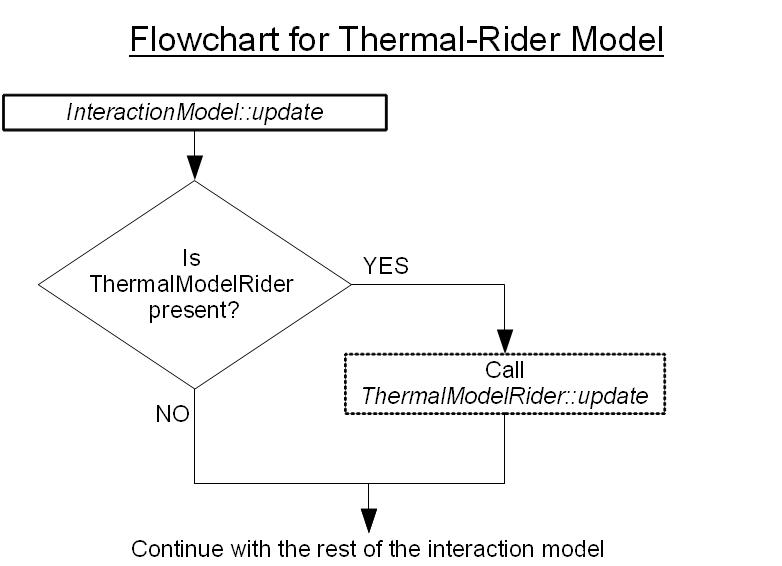
\includegraphics[height=3.8in]{figures/flow_chart_1.jpg}
\caption{Illustration of how the \ThermalRiderDesc\ is incorporated
into the simulation.}
\label{fig:thermalflowchart1}
\end{center}
\end{figure}

\begin{figure}[htp]
\begin{center}
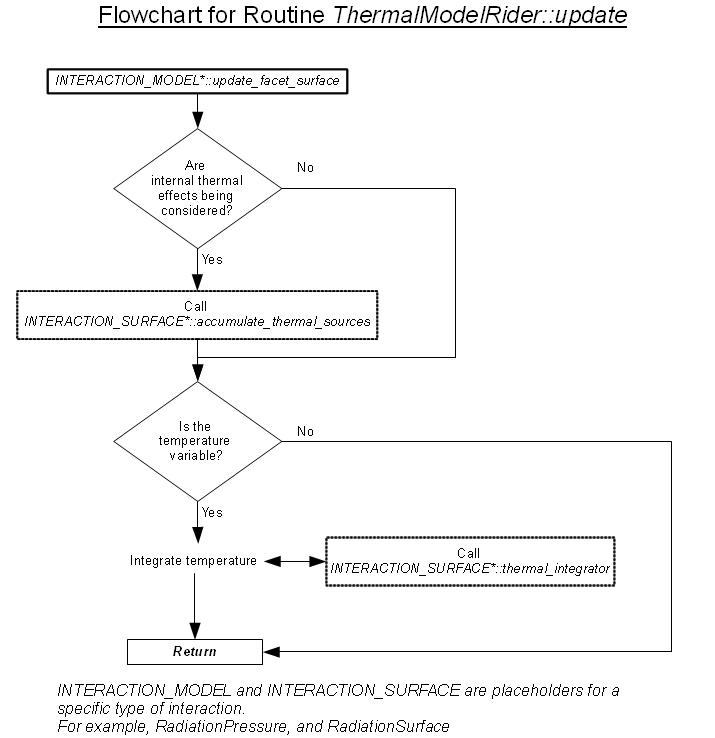
\includegraphics[height=7.2in]{figures/flow_chart_tmr_update.jpg}
\caption{The \ThermalRiderDesc\ controls the calls to the
interaction surface.}
\label{fig:thermalflowchart1a}
\end{center}
\end{figure}

\begin{figure}[htp]
\begin{center}
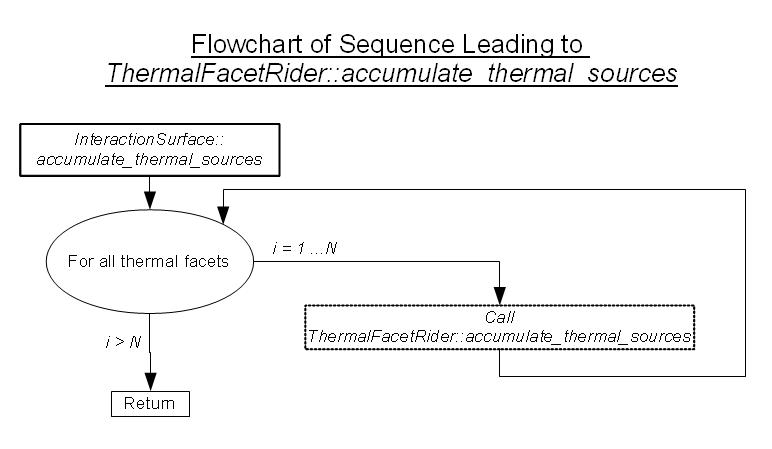
\includegraphics[height=3.9in]{figures/flow_chart_2.jpg}
\caption{The Interaction Surface controls the calls to each of the
interaction facets to independently accumulate the thermal sources on
that facet.}
\label{fig:thermalflowchart2}
\end{center}
\end{figure}

\begin{figure}[htp]
\begin{center}
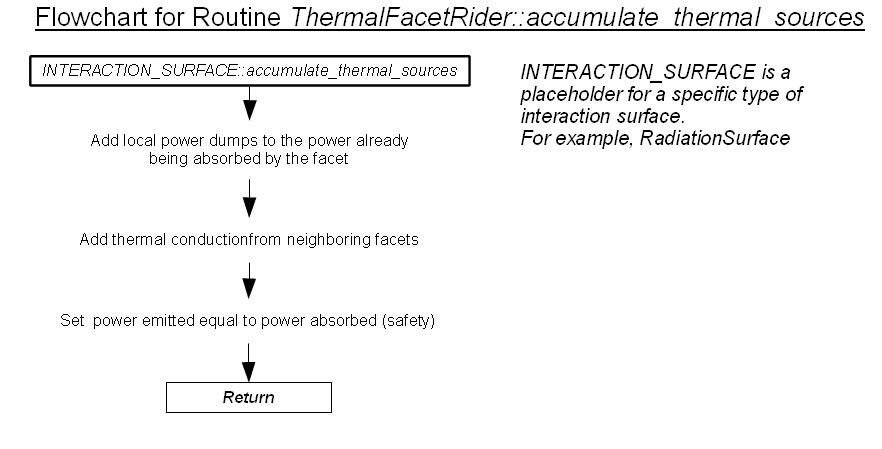
\includegraphics[height=3.4in]{figures/flow_chart_tfr_ats.jpg}
\caption{Each facet uses the functionality contained within its
thermal rider to collect (calculating where necessary) the thermal
sources being absorbed by that surface.}
\label{fig:thermalflowchart3}
\end{center}
\end{figure}

\begin{figure}[htp]
\begin{center}
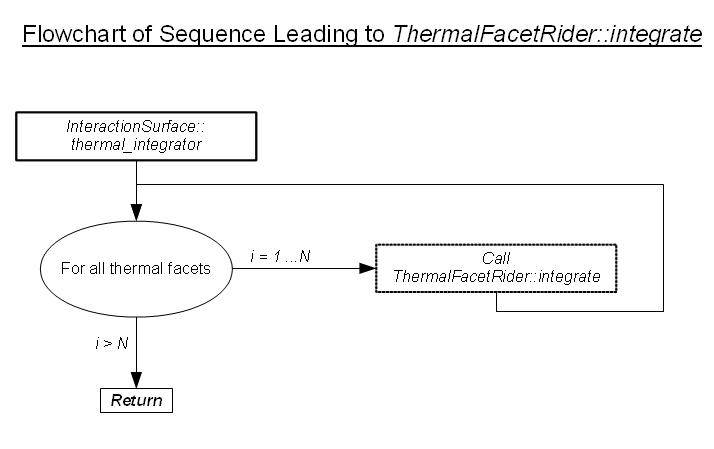
\includegraphics[height=4in]{figures/flow_chart_4.jpg}
\caption{The interaction surface controls the calls to each of the
interaction facets to independently integrate the rate of change of
temperature resulting from the accumulated thermal sources.} 
\label{fig:thermalflowchart4}
\end{center}
\end{figure}

\begin{figure}[htp]
\begin{center}
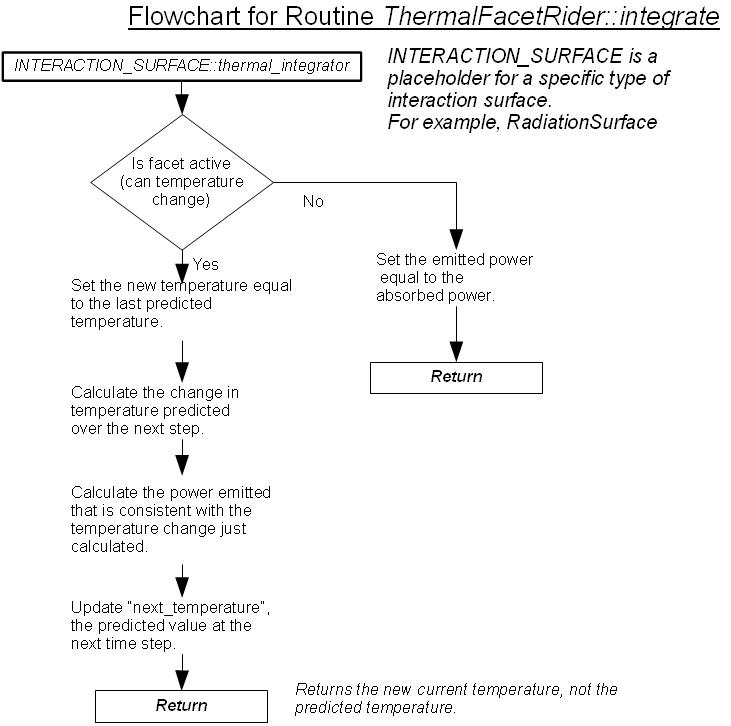
\includegraphics[height=6in]{figures/flow_chart_tfr_integrate.jpg}
\caption{Each facet uses the functionality contained within its 
thermal rider to integrate the temperature variation across one
integration step, and from that, determine the mean rate at which
thermal radiation was emitted.}
\label{fig:thermalflowchart5}
\end{center}
\end{figure}




\clearpage

\subsection{Functional Design}
See the \href{file:refman.pdf}{Reference Manual}\cite{thermalbib:ReferenceManual} for a summary of member data and member methods for all classes.  This section describes the functional operation of the methods in each class.

Objects are presented in alphabetical order.
Methods are presented in alphabetical order within the object in
which they are located.  

\begin{enumerate}
\classitem{ThermalFacetRider} Base-class

This is the rider that attaches to a particular instance of the
generic and virtual InteractionFacet object.

{\bf Methods:}

\begin{enumerate}

\funcitem{accumulate\_thermal\_sources}\label{ref:facetaccumulatethermalsources}

It is assumed that any external, model-specific, heating sources have
already been accumulated (e.g., as a result of radiative absorption
(\textit{radiation\_pressure}), or aerodynamic drag heating
(\textit{aerodynamics})).  This method is intended to be used to
accumulate vehicular sources of energy, such as a power sink/source
from within the vehicle, or conduction between facets.

\funcitem{initialize}\label{ref:facetinitialize}
When the facet is initialized, we set both the
\textit{dynamic\_temperature}
(that is the operating temperature) and the
\textit{next\_temperature} (the operating temperature predicted at
the end of the current integration step) to the initialization value.

The radiative emission, known from equation \ref{eqn:thermalemission} to be 
$P_{emit} = \epsilon \sigma A T^4$ must be
calculated repeatedly.  Three of those values are constants, so those
are stored together in a new variable, \textit{rad\_constant
=}$\epsilon \sigma A$.


\funcitem{integrate}\label{ref:facetintegrate}
The integration routine is described in detail in the
\textref{integrator}{ref:thermalRK4integrator} description found in
the Mathematical Formulation section of this document.
\end{enumerate}


\classitem{ThermalIntegrableObject}er7\_utils::IntegrableObject 

This is a derived class of a generic object specialized for thermal
integration which can be integrated by JEOD.

{\bf Methods:}

\begin{enumerate}

\funcitem{compute\_temp\_dot}\label{ref:integratecomputetempdot}
Computes the time derivative of temperature and the 
instantaneous rate of emission.

\funcitem{create\_integrators}\label{integratecreateintegrators}
Required by \textit{er7\_utils::IntegrableObject}


\funcitem{destroy\_integrators}\label{integratedestroyintegrators}
Required by \textit{er7\_utils::IntegrableObject}


\funcitem{initialize}\label{ref:integrateinitialize}
Sets the initial temperature and caches a pointer to the
\textit{ThermalFacetRider} associated with the facet to be integrated.


\funcitem{integrate}\label{ref:integrateintegrate}
Implements the \textit{integrate} method of 
\textit{er7\_utils::IntegrableObject}


\funcitem{get\_temp}\label{integrategettemp}
Accessor method for the temperature

\funcitem{get\_temp\_dot}\label{integrategettempdot}
Accessor method for time derivative of temperature.


\funcitem{reset\_integrators}\label{integrateresetintegrators}
Required by \textit{er7\_utils::IntegrableObject}
\end{enumerate}


\classitem{ThermalMessages}
  Base-class

This is the message handler for the \ThermalRiderDesc.  It has
no methods.



\classitem{ThermalModelRider}
  Base-class

This is the object that rides on the interaction model directly.


{\bf Methods:}

\begin{enumerate}
\funcitem{update}
If the model is to include thermal sources coming from within the
vehicle, the \textit{model} method \textit{accumulate\_thermal\_sources} is called,
which ultimately calls the \textit{facet} method
\textref{accumulate\_thermal\_sources}{ref:facetaccumulatethermalsources}
for each of the facets.

If the temperature of the surface is intended to be dynamic, the
routine \textit{thermal\_integrator} is called
which ultimately calls 
\textref{integrate}{ref:facetintegrate} for each of the facets.
\end{enumerate}

\classitem{ThermalParams}
  Base-class

This class contains the collection of data for a thermal facet; it
contains no methods.


\end{enumerate}




%\section{Version Inventory}
%%%%%%%%%%%%%%%%%%%%%%%%%%%%%%%%%%%%%%%%%%%%%%%%%%%%%%%%%%%%%%%%%%%%%%%%%%%%%%%%%
%
% Purpose:  Inventory of files for the time model
%
% 
%
%%%%%%%%%%%%%%%%%%%%%%%%%%%%%%%%%%%%%%%%%%%%%%%%%%%%%%%%%%%%%%%%%%%%%%%%%%%%%%%%


\section{Inventory}
All \ThermalRiderDesc\ files are located in the directory \newline
{\tt \$\{JEOD\_HOME\}/models/interactions/thermal\_rider}.
Relative to this directory,
\begin{itemize}
\vspace{-0.2\baselineskip}
\item Header and source files are located
in the model {\tt include} and {\tt src} subdirectories.
Table~\ref{tab:source_files} lists the
configuration-managed files in these directories.
\vspace{-0.1\baselineskip}
\item Documentation files are located in the model {\tt docs} subdirectory.
See table~\ref{tab:documentation_files}
for a listing of the
configuration-managed files in this directory.
\vspace{-0.1\baselineskip}
\item Verification files are located in the model {\tt verif} subdirectory.
See table~\ref{tab:verification_files}
for a listing of the
configuration-managed files in this directory.
\end{itemize}

\input{inventory}


\chapter{User's Guide}\hyperdef{part}{user}{}\label{ch:user}
%----------------------------------
The User's Guide is divided into 3 components, one for each of three
different types of user.

The Analysis section of the User's Guide is intended primarily for
users of pre-existing simulations.
It comprises the following elements:
\begin{itemize}
\item A description of how to modify \ThermalRiderDesc\ variables after
the simulation
has compiled, including an in-depth discussion of the input file;
\item An overview of how to interpret (but not edit) the S\_define
file;
\item A sample of some of the typical variables that may be logged.
\end{itemize}

The Integration section of the User's Guide is intended for simulation
developers.
It describes the necessary configuration of the \ThermalRiderDesc\
within an
S\_define file, and the creation of standard run directories.  The
latter
component assumes a thorough understanding of the preceding Analysis
section of the user guide.
Where applicable, the user may be directed to selected portions of
Product Specification (Chapter \ref{ch:spec}).

The Extension section of the User's Guide is intended primarily for
developers
needing to extend the capability of the \ThermalRiderDesc.  Such users
should have a
thorough understanding of how the model is used in the preceding
Integration section, and of the model
specification (described in Chapter \ref{ch:spec}).


\section{Analysis}
%%%%%%%%%%%%%%%%%%%%%%%%%%%%%%%%%%%%%%%%%%%%%%%%%%%%%%%%%%%%%%%%%%%%%%%%%%%%%%%%%
%
% Purpose:  Analysis part of User's Guide for the ThermalRider model
%
% 
%
%%%%%%%%%%%%%%%%%%%%%%%%%%%%%%%%%%%%%%%%%%%%%%%%%%%%%%%%%%%%%%%%%%%%%%%%%%%%%%%%

% \section{Analysis}
\label{sec:user_analysis}
Determining whether or not the \ThermalRiderDesc\ is included in a simulation is
non-obvious; because the model rides on some other model, it is unlikely to
appear as an \textit{S\_define} file entry.  Instead, it is necessary to look
for the data files that are used to define the vehicle surface.  An example of
this is found in the radiation pressure model, at \newline
\textit{interactions/radiation\_pressure/verif/SIM\_2\_SHADOW\_CALC/SET\_test/RUN\_ten\_plates/input} \newline
(here, the \ThermalRiderDesc\ is riding on the Radiation Pressure Model).  We will use this example as a guide to establishing the Thermal Rider on any model.

At some point in any simulation that utilizes a surface-interaction, the surface must be defined; that definition is typically carried out through a data file.  There may also be some values that are set in the input file.  This particular input file contains the surface description at the very end, and includes the data file \textit{Modified\_data/radiation\_surface\_v2.d}, which defines the surface.  Simple models, with only one surface, may put all of the thermal characteristics into the input file (e.g., \textit{interactions/radiation\_pressure/verif/SIM\_1\_BASIC/SET\_test/RUN\_basic/input}, which includes a data file for the full surface, and just a few lines for the default spherical surface).

The \ThermalRiderDesc\ descriptors fall into one of three categories:
\begin{itemize}
\item  The model-wide descriptors.
\item The facet-specific descriptors.
\item The facet parameter descriptors (material-specific).  
\end{itemize}
The facets are the sections of the overall vehicle surface into which that surface has been divided; they are defined and controlled at an individual level.

\subsection{Model-wide Descriptors}
These values are found one level below the thermal rider, which is one level
below the interaction model on which the \ThermalRiderDesc\ rides, e.g.,
\textit{radiation.rad\_pressure.thermal.***}.

\begin{itemize}
\item{\textit{active}}\ \newline
The \textit{active} flag toggles the entire \ThermalRiderDesc\ on or off.  The default value is \textit{false} (i.e., off).  This flag would typically be set in an input file, or in the case of the Radiation Pressure Model (upon which we are currently riding), this flag is automatically set to true, since the Radiation Pressure Model cannot function without a Thermal Rider.  
\item{\textit{include\_internal\_thermal\_effects}}\ \newline
This flag allows for the inclusion of thermal flow within the vehicle, e.g., from a power source inside the vehicle, or facet-to-facet conduction.  This flag also defaults to \textit{false}.
\end{itemize}

\subsection{Facet-specific Descriptors}
These values are found one level below the thermal rider, which is one level
below the facet on which it rides, which is one level below the surface, e.g.,
\textit{radiation.rad\_surface.facets.thermal.***}
\begin{itemize}
\item{\textit{active}}\ \newline
In addition to having the capability to turn the entire thermal model on or off, facets are equipped with an individual on/off flag to indicate whether or not to integrate the temperature.  A facet that is inactive ($active = false$) will just retain a constant temperature.
\item{\textit{heat\_capacity}}\ \newline
This can be defined for the facet at an individual level, or in the parameters list as a heat capacity per unit area (a material property), which is then converted into the facet-specific \textit{heat\_capacity} by functionality within the model-specific Interaction Facet.
\item{\textit{thermal\_power\_dump}}\ \newline
This value allows some level of thermal power to be transfered to the facet from within the vehicle if the model-wide \textit{include\_internal\_thermal\_effects} flag is set.  A positive value represents flow into the facet, a negative value represents flow out of the facet.
\end{itemize}


\subsection{Facet Parameter Descriptors}
These values describe the material with which a facet is made.  Each facet is assigned a parameter list; this avoids repetition of identical information from facet to facet.  In our example, only one material is defined, \textit{radiation\_test\_material}, and it is assigned to all facets.
\begin{itemize}
\item{\textit{emissivity}}\ \newline
The emissivity measures how similar to a black-body a material is in the thermal emission that it gives off.  An emissivity of 1.0 represents a perfect black-body, an emissivity of 0.0 implies that the surface cannot radiate at all.
\item{\textit{heat\_capacity\_per\_area}}\ \newline
This is converted into the facet-specific \textit{heat capacity} by functionality within the model-specific Interaction Facet.  It is useful to allow for comparable behavior across facets of vastly different size without the necessity of calculating the heat capacity for each facet individually.
\end{itemize}


%\section{Integration}
%%%%%%%%%%%%%%%%%%%%%%%%%%%%%%%%%%%%%%%%%%%%%%%%%%%%%%%%%%%%%%%%%%%%%%%%%%%%%%%%%
%
% Purpose:  Integration part of User's Guide for the ThermalRider model
%
% 
%
%%%%%%%%%%%%%%%%%%%%%%%%%%%%%%%%%%%%%%%%%%%%%%%%%%%%%%%%%%%%%%%%%%%%%%%%%%%%%%%%

 \section{Integration}
 \label{sec:user_integration}

Including the Thermal Rider option into any existing surface is fairly straightforward, the most difficult part of using the \ThermalRiderDesc\ is in creating the \textit{Interaction Surface} on which it will ride.  The \ThermalRiderDesc\ comes in two parts, one attached to each of the facets, and one attached to the interaction model itself (the \textit{thermal facet rider} and \textit{thermal model rider} respectively).  We will treat these individually.  If the interaction model does not include both the model rider and the facet riders, see the section \textref{Extension}{sec:user_extension} for details on how to extend an interaction model to include the Thermal Rider.

\subsection{\ThermalRiderDesc}
The main class for the interaction model (e.g. \textit{RadiationPressure} for the Radiation Pressure Model) must contain an instance of the \ThermalRiderDesc.
Every Interaction Model must already have an \textit{update} (or similar) method, through which the interaction forces are updated.  This method must call the \textit{thermal.update} method (\textit{thermal} being the name of the instance of the \ThermalRiderDesc).  The setting of data values necessary to the \ThermalRiderDesc\ is covered in the section \textref{Analysis}{sec:user_analysis}.



\subsection{Thermal Facet Rider}
This rider must be attached to each of the facets in the surface; ideally, the thermal rider would be added when the model-specific interaction facets are defined, based on the generic Interaction Facet.  See, for an example. the class \textit{RadiationFacet} in the Radiation Pressure Model. 

It is important to ensure that all facets in the surface have thermal characteristics available to them, even if the intention is to de-activate the thermal activity in many of those facets.  The code is expecting that certain methods will be available to all facets, and that will only work if they all contain the Thermal Facet Rider.

Setting the data for the each of the facets is covered in section \textref{Analysis}{sec:user_analysis}.









%\section{Extension}
%%%%%%%%%%%%%%%%%%%%%%%%%%%%%%%%%%%%%%%%%%%%%%%%%%%%%%%%%%%%%%%%%%%%%%%%%%%%%%%%%
%
% Purpose:  Extension part of User's Guide for the ThermalRider model
%
% 
%
%%%%%%%%%%%%%%%%%%%%%%%%%%%%%%%%%%%%%%%%%%%%%%%%%%%%%%%%%%%%%%%%%%%%%%%%%%%%%%%%

 \section{Extension}
 \label{sec:user_extension}

\subsection{Extending the Capability of the \ThermalRiderDesc.}
The \ThermalRiderDesc\ is intended to be a stand-alone sub-model, used to enhance an interaction model.  There is no specific plan to extend the capability of the \ThermalRiderDesc.

\subsection{Using the \ThermalRiderDesc\ to Extend the Capability of an Interaction Model.}

The \ThermalRiderDesc\ comes in two parts, one attached to each of the facets, and one attached to the interaction model itself (the \textit{thermal facet rider} and \textit{thermal model rider} respectively).  Both must be added to the interaction model in order for the \ThermalRiderDesc\ to function.  We will treat these individually.

\subsection{\ThermalRiderDesc}
\begin{enumerate}
\item
If the main class for the interaction model (e.g. \textit{RadiationPressure} for the Radiation Pressure Model) does not contain an instance of the \ThermalRiderDesc, add one.  Call it \textit{thermal.}
\item
Every Interaction Model must already have an \textit{update} (or similar) method, through which the interaction forces are updated.  This method must perform the following additional tasks:
\begin{enumerate}
\item Call the \textit{thermal.update} method (\textit{thermal} being the name of the instance of the \ThermalRiderDesc).  This may require the addition of code to the interaction model update method; if so use the Radiation Pressure Model as a template. 
\item Obtain the integration step size that will be used by the thermal integrator.  Again, use the Radiation Pressure model as a template.
\end{enumerate}
\item
It is assumed that if the user makes the effort to specify the \ThermalRiderDesc, that the intention is to have it active.  The \textit{model-level} active flag therefore defaults to \textit{true} (i.e., on).
\end{enumerate}


\subsection{Thermal Facet Rider}
Adding the Facet Rider is more complicated than adding the Model Rider.  Since the interaction surface comprises the facets, changing the facets requires changes to the interaction surface.

\subsubsection{Thermally Active Facets}
\begin{enumerate}
\item
When the facet is created, the thermal values from the parameter list must be copied over into the facet (see \textit{RadiationFacet::define\_facet\_core}).
\item
Within the initialization of the Interaction Facet, the \textit{thermal.initialize} method must be called; this sets the radiation constant that is used in modeling the thermal radiation, and initializes the dynamic and next-step temperatures.
\item
If the interaction force is temperature dependent, the thermal integrator must be called from some method that is called at the regular update rate in order to maintain the correct temperature profile.  Note that it is the thermal integration method that updates \textit{thermal.dynamic\_temperature} to the value calculated in the previous integration step, so this method should be called before the \textit{current} temperature is needed.
\end{enumerate}

\subsubsection{Thermally Active Surface}
The thermally active surface should contain the following additional methods:
\begin{enumerate}
\item{accumulate\_thermal\_sources}
\item{thermal\_integrator}
\item{equalize\_absorption\_emission}
\end{enumerate}
These are simple interface methods, passing control from the model through to the individual facets one at a time.  They can typically be copied verbatim from the example of a Radiation Surface in the Radiation Pressure model.




%----------------------------------
\chapter{Verification and Validation}\hyperdef{part}{ivv}{}\label{ch:ivv}
%----------------------------------

\section{Verification}
%%%%%%%%%%%%%%%%%%%%%%%%%%%%%%%%%%%%%%%%%%%%%%%%%%%%%%%%%%%%%%%%%%%%%%%%%%%%%%%%%
%
% Purpose:  Verification part of V&V for the ThermalRider model
%
% 
%
%%%%%%%%%%%%%%%%%%%%%%%%%%%%%%%%%%%%%%%%%%%%%%%%%%%%%%%%%%%%%%%%%%%%%%%%%%%%%%%%

% \section{Verification}

%%% code imported from old template structure
%\inspection{<Name of Inspection>}\label{inspect:<label>}
% <description> to satisfy  
% requirement \ref{reqt:<label>}.
\subsection{Inspections}

\inspection{Top-level Inspection}\label{inspect:top_level}
This document, the code, and associated files, have been inspected, and together
satisfy requirement~\ref{reqt:top_level}.

\inspection{Extended Functionality} \label{inspect:thermal_ext_func}
The method \textit{ThermalFacetRider::accumulate\_thermal\_sources} includes the
functionality to add thermal power sources or sinks (see \textref{Verification
of Intra-vehicular Thermal Transfer}{test:intravehicularthermaltransfer}), and a good description of how a conduction model could be implemented.  The addition of heating due to aerodynamic drag has not been investigated in depth, but it is anticipated that this would be handled by the aerodynamics model by adding a Thermal Rider to the existing aerodynamics model.  This satisfies requirement~\ref{reqt:thermal_ext_func}



\subsection{Verification of the Temperature Modeling}
\label{test:temperature}

  The simulations for this verification procedure are found in the Radiation Pressure model; this verification test is duplicated in the Radiation Pressure model.
  
  This section is divided into two parts, one comparing the case of
  the vehicle without illumination --- for which an analytic solution
  exists --- and the second comparing the response of surfaces with different
  characteristics in the presence of illumination.

  \subsubsection{Verification of thermal processes without illumination}
  \test{Thermal Processes - no illumination}
  \label{test:temperature_integration1}
  \begin{description}
  \item{Purpose:}\ \newline
    This test is to ensure that the Runge-Kutte plate-temperature integration
    process is functioning normally in the case of a vehicle cooling in the
    absence of incident radiation.
  \item{Requirements:}\ \newline
    Satisfactory conclusion of this test, along with test~\ref{test:temperature_integration2} satisfies requirements~\ref{reqt:temp_monitoring} and~\ref{reqt:thermal_min_func}.
  \item{Procedure:}\ \newline
    The simulation used in this test is available at \newline
    \textit{radiation\_pressure/verif/SIM\_2\_SHADOW\_CALC/RUN\_shadow\_cooling}.
    A number of facets were monitored in a flux-free environment to observe
    their temperature variation with time.  Each plate had
    slightly different characteristics, allowing for the dependency on
    emissivity, plate area, and heat capacity to be investigated.  In the
    absence of incident flux, an analytic solution exists for the temperature
    and the force, and this can be compared to the numerical solution.
  \item{Results:}
    \begin{enumerate}
    \item{Variation with time of temperature}\newline
      Simulation data of the variation with time of temperature matched very well to analytic solution.  On any scale
      longer than 3 timesteps, the graphs of analytical values and simulation
      values were indistinguishable, with a difference less than 0.05\%, and
      very much smaller than the observed changes in temperature.  See Figure~\ref{fig:temperatureanalytic}.
      \begin{figure}[!ht]
         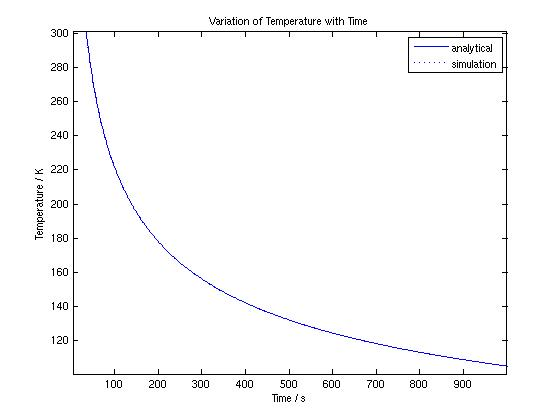
\includegraphics[width=180mm]{figures/temperature_analytic.jpg}
         \caption{Variation of Temperature with time showing the simulation data
         and analytic solution overlaying.}
         \label{fig:temperatureanalytic}
      \end{figure}
    \item{Variation with emissivity of the temporal evolution of temperature}\newline
      As the emissivity increases, the rate of change of temperature also
      increases, as expected.  For $\epsilon$=0, no temperature
      change was observed.
    \item{Variation with starting temperature of the temporal evolution of temperature}\newline
      With a lower starting temperature, a plate maintains a lower temperature
      throughout the simulation, but the temperature decreases more slowly.
      Temperature$\sim$time plots have identical shapes; shifting the curves along
      the x-axis to match temperature at some time results in matching
      temperatures for all (valid) time.
    \item{Variation with plate area of the temporal evolution of temperature}\newline
      A plate with a smaller surface area, but identical heat capacity shows a
      more gradual temperature drop.  There is no observable difference between
      plates for which the heat capacity is decreased proportionally with the 
      area (e.g. smaller plate of the same material). 
    \item{Variation with heat capacity of the temporal evolution of temperature}\newline
      A plate with a smaller heat capacity, but identical area shows a
      more rapid temperature drop.  There is no observable difference between
      plates for which the area is decreased proportionally with the heat 
      capacity (e.g. smaller plate of the same material). 
    \end{enumerate}
    
  \end{description}
  \clearpage

  \subsubsection{Verification of thermal processes with illumination}
  \test{Thermal Processes - with illumination}
  \label{test:temperature_integration2}
  \begin{description}
  \item{Purpose:}\ \newline
    To verify that the temperature integration and thermal emission processes
    are functioning as expected when the vehicle is illuminated.
  \item{Requirements:}\ \newline
    Satisfactory conclusion of this test, along with test~\ref{test:temperature_integration1} satisfies requirements~\ref{reqt:temp_monitoring} and~\ref{reqt:thermal_min_func}.
    
  \item{Procedure:}\ \newline
  The simulation used in this test is available at \textit{SIM\_2\_SHADOW\_CALC/RUN\_ten\_plates}.
    10 identical plates were oriented at different angles to the flux
    vector, with the angle between the normal and the flux vector varying
    from 0 to 90 degrees.  All plates were started with a preliminary
    temperature of 270 K, and the simulation was allowed to run until all but
    one plate had approached their equilibrium temperature.  The force from each plate
    was monitored throughout the simulation. 
  \item{Results:}\ \newline
    The equilibrium temperature is calculated from the energy balance equation
    \begin{equation}
      \phi (A\cos \theta )(1-\alpha )=\epsilon \sigma A{T_{\mathit{eq}}}^{4}
    \end{equation}
        
    where
    \begin{itemize}
      \item{} 
        $\phi$ is the radiative flux, 
      \item{} 
        $\theta$ is the angle between the surface normal and the incident
        radiation vector, 
      \item{}
        $\alpha$ is the albedo of the surface, 
      \item{}
        $\epsilon$ is the emissivity of the surface, 
      \item{}
        $\sigma$ is the Stefan-Boltzmann constant, 
      \item{}
        A is the plate area, and
      \item{}  
        $T_{\mathit{eq}}$ is the equilibrium temperature.
    \end{itemize}

    Using values of $\alpha =0.5$,  $\epsilon =0.5$, $\phi =
    1400~W~ m^{-2}$, and with $\theta$ varying from 0 to 90 degrees in 10 degree 
    intervals, the equilibrium temperatures of the 10 plates are:

    396 K, 395 K, 390 K, 382 K, 371 K, 355 K, 333 K, 303 K, 256 K, and 0 K.
    
    Figure~\ref{fig:ivv_F_emission_Tint} shows the variation with time of the
    temperature of the 10 plates; the 9 plates that had closely approached equilibrium temperatures had 
    final temperatures all within
    1\% of their analytical equilibrium temperature.  The final plate, with an equilibrium temperature of 0 K has a temperature
    variation that is decreasing at a rate consistent with expectations.
    
      \begin{figure}[!ht]
        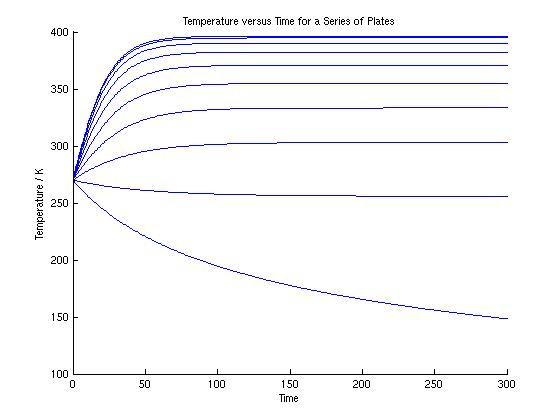
\includegraphics[width=180mm]{figures/temperature-time.jpg}
        \caption{The variation of temperature with time over the 10 plates in
        the simulation.} 
        \label{fig:ivv_F_emission_Tint}
      \end{figure}
  \end{description}
    

    
\clearpage

\test{Verification of Intra-vehicular Thermal Transfer} \label{test:intravehicularthermaltransfer}
\begin{description}
\item{Purpose:}\newline
To test the capability of modeling thermal energy transfer from within the vehicle to the surface.
\item{Requirements:}\newline
Satisfactory conclusion of this test, together with inspection \ref{inspect:thermal_ext_func} satisfies requirement \ref{reqt:thermal_ext_func}
\item{Procedure:}\newline
A test comparable to the basic Radiation Pressure test \newline
(\textit{interactions/radiation\_pressure/verif/SIM\_1\_BASIC/RUN\_basic}) was
performed (at \textit{interactions/radiation\_pressure/verif/SIM\_1\_BASIC/RUN\_thermal\_dump}).  The difference being that in this test, a thermal power dump sufficient to raise the temperature of the surface by 1 degree per second was added.
\item{Predictions:}\newline
The temperature of the surface should initially rise by 1 degree per second above the temperature of the surface without the thermal power input.  As radiative cooling increases in response, the rate of change should diminish over time; eventually a new equilibrium will be reached at some higher temperature than the case with no thermal power dump.
\item{Results:}\newline
The results were as expected; after 1 second, the temperature difference was 0.985 degrees; after 2 seconds, 1.94 degrees (0.97 degrees per second average); after 10 seconds, 8.6 degrees (0.86 degrees per second average); after 25 seconds, 17 degrees (0.68 degrees per second average).

\end{description}


%\section{Validation}
%%%%%%%%%%%%%%%%%%%%%%%%%%%%%%%%%%%%%%%%%%%%%%%%%%%%%%%%%%%%%%%%%%%%%%%%%%%%%%%%%
%
% Purpose:  Validation part of V&V for the ThermalRider model
%
% 
%
%%%%%%%%%%%%%%%%%%%%%%%%%%%%%%%%%%%%%%%%%%%%%%%%%%%%%%%%%%%%%%%%%%%%%%%%%%%%%%%%

\section{Validation}

%%% code imported from old template structure
%\test{<Title>}\label{test:<label>}
%\begin{description}
%\item[Purpose:] \ \newline
%<description>
%\item[Requirements:] \ \newline
%By passing this test, the universal time module 
%partially satisfies requirement~\ref{reqt:<label1>} and 
%completely satisfies requirement~\ref{reqt:<label2>}.
%\item[Procedure:]\ \newline
%<procedure>
%\item[Results:]\ \newline
%<results>
%\end{description}

There is no independent validation of the \ThermalRiderDesc.

\section{Metrics}
\subsection{Code Metrics}

Table~\ref{tab:coarse_metrics} presents coarse metrics on the
source files that comprise the model.

\input{coarse_metrics}

Table~\ref{tab:metrix_metrics} presents the extended cyclomatic
complexity
(ECC) of the methods defined in the model.
\input{metrix_metrics}


%%%%%%%%%%%%%%%%%%%%%%%%%%%%%%%%%%%%%%%%%%%%%%%%%%%%%%%%%%%%%%%%%%%%%%%%%
% Bibliography
%%%%%%%%%%%%%%%%%%%%%%%%%%%%%%%%%%%%%%%%%%%%%%%%%%%%%%%%%%%%%%%%%%%%%%%%%
\newpage
\pdfbookmark{Bibliography}{bibliography}
\bibliography{dynenv,ThermalRider}
\bibliographystyle{plain}

%\pagebreak
%\appendix

\end{document}
